\section{Qsim::VmQMemOp Struct Reference}
\label{structQsim_1_1VmQMemOp}\index{Qsim::VmQMemOp@{Qsim::VmQMemOp}}
{\tt \#include $<$qsim.h$>$}

Inheritance diagram for Qsim::VmQMemOp:\nopagebreak
\begin{figure}[H]
\begin{center}
\leavevmode
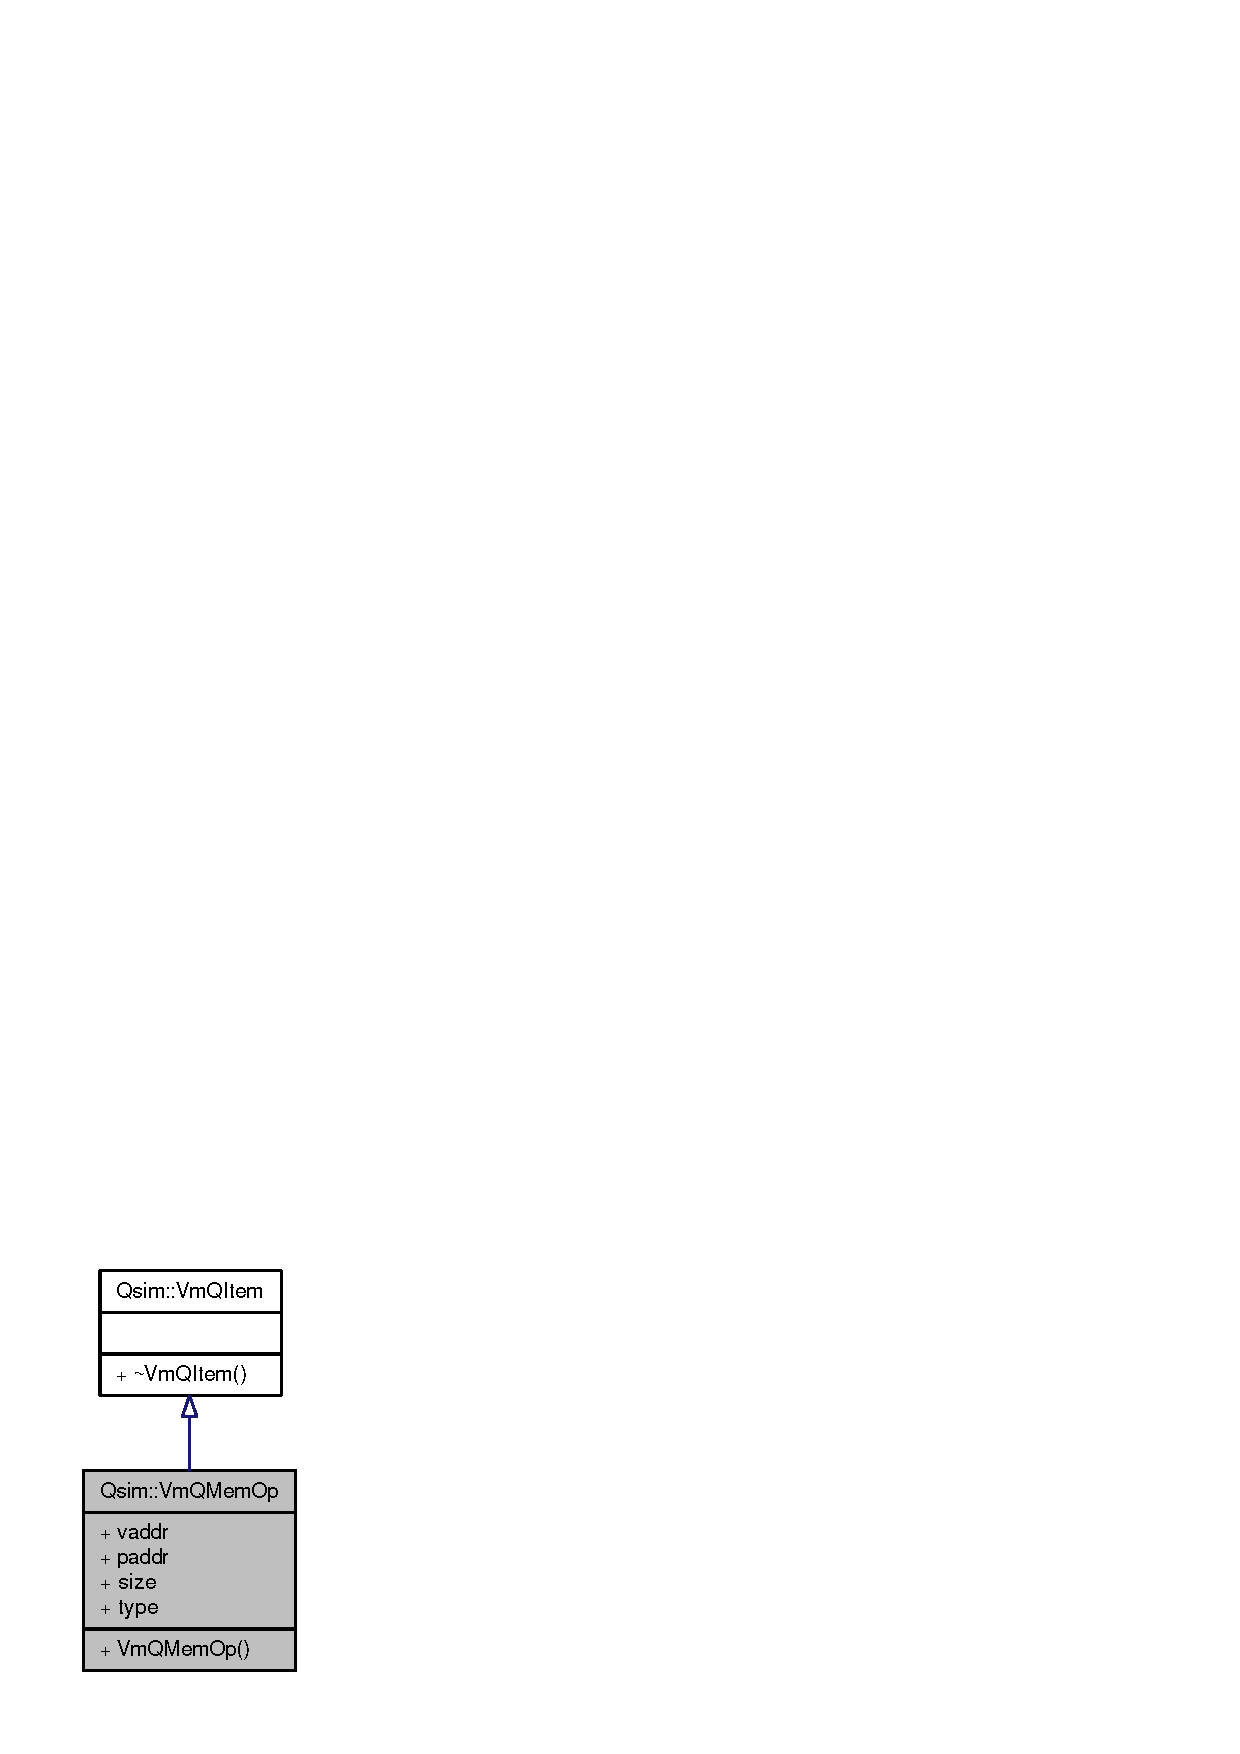
\includegraphics[width=146pt]{structQsim_1_1VmQMemOp__inherit__graph}
\end{center}
\end{figure}
Collaboration diagram for Qsim::VmQMemOp:\nopagebreak
\begin{figure}[H]
\begin{center}
\leavevmode
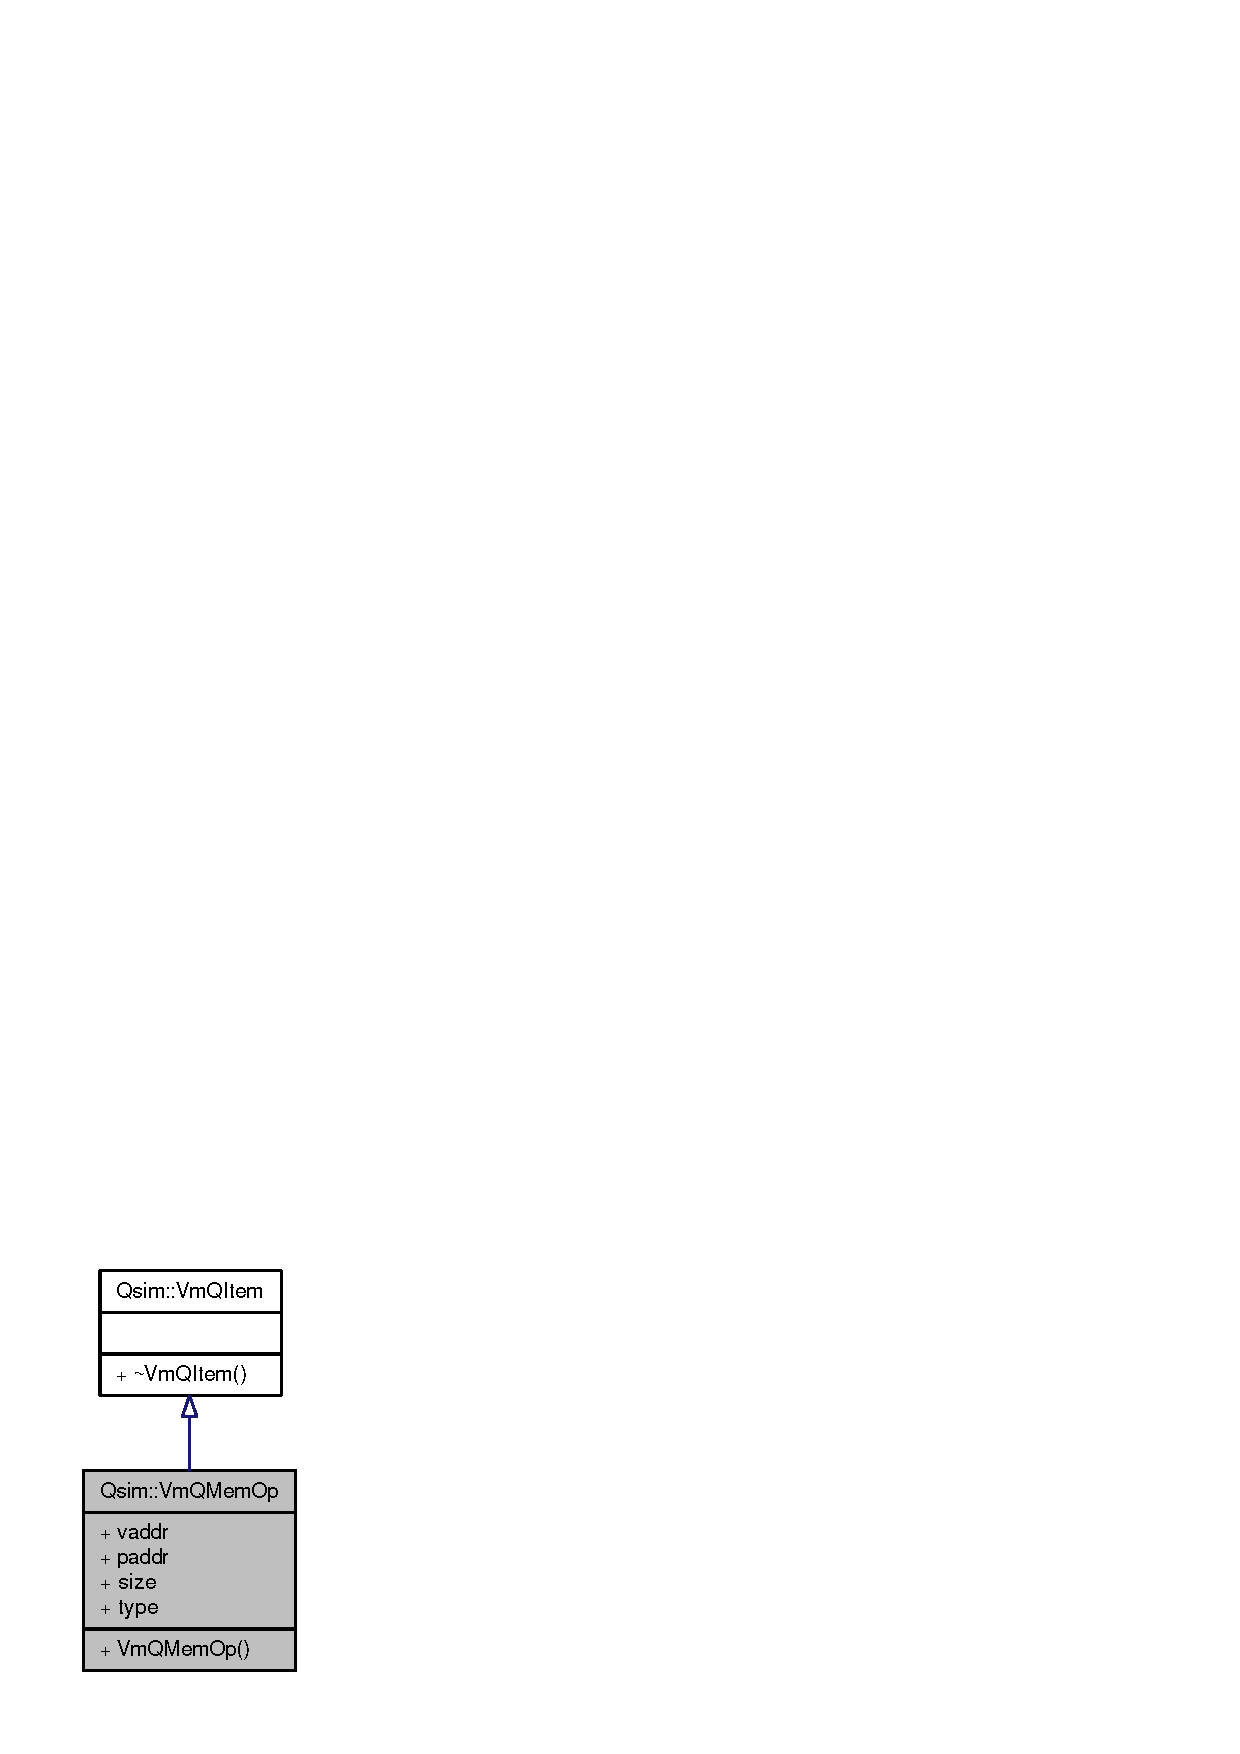
\includegraphics[width=146pt]{structQsim_1_1VmQMemOp__coll__graph}
\end{center}
\end{figure}
\subsection*{Public Member Functions}
\begin{CompactItemize}
\item 
{\bf VmQMemOp} (uint64\_\-t {\bf vaddr}, uint64\_\-t {\bf paddr}, uint8\_\-t {\bf size}, {\bf MemOpType} {\bf type})
\end{CompactItemize}
\subsection*{Public Attributes}
\begin{CompactItemize}
\item 
uint64\_\-t {\bf vaddr}
\item 
uint64\_\-t {\bf paddr}
\item 
uint8\_\-t {\bf size}
\item 
{\bf MemOpType} {\bf type}
\end{CompactItemize}


\subsection{Detailed Description}


Definition at line 106 of file qsim.h.

\subsection{Constructor \& Destructor Documentation}
\index{Qsim::VmQMemOp@{Qsim::VmQMemOp}!VmQMemOp@{VmQMemOp}}
\index{VmQMemOp@{VmQMemOp}!Qsim::VmQMemOp@{Qsim::VmQMemOp}}
\subsubsection[{VmQMemOp}]{\setlength{\rightskip}{0pt plus 5cm}Qsim::VmQMemOp::VmQMemOp (uint64\_\-t {\em vaddr}, \/  uint64\_\-t {\em paddr}, \/  uint8\_\-t {\em size}, \/  {\bf MemOpType} {\em type})\hspace{0.3cm}{\tt  [inline]}}\label{structQsim_1_1VmQMemOp_de2be2afe65bda8fc428997880df84ac}




Definition at line 107 of file qsim.h.

\subsection{Member Data Documentation}
\index{Qsim::VmQMemOp@{Qsim::VmQMemOp}!paddr@{paddr}}
\index{paddr@{paddr}!Qsim::VmQMemOp@{Qsim::VmQMemOp}}
\subsubsection[{paddr}]{\setlength{\rightskip}{0pt plus 5cm}uint64\_\-t {\bf Qsim::VmQMemOp::paddr}}\label{structQsim_1_1VmQMemOp_291b6e2d4e0592933eb2638520b1395e}




Definition at line 109 of file qsim.h.\index{Qsim::VmQMemOp@{Qsim::VmQMemOp}!size@{size}}
\index{size@{size}!Qsim::VmQMemOp@{Qsim::VmQMemOp}}
\subsubsection[{size}]{\setlength{\rightskip}{0pt plus 5cm}uint8\_\-t {\bf Qsim::VmQMemOp::size}}\label{structQsim_1_1VmQMemOp_6e161d6ad6e0818f4a8624236e60b4d1}




Definition at line 110 of file qsim.h.\index{Qsim::VmQMemOp@{Qsim::VmQMemOp}!type@{type}}
\index{type@{type}!Qsim::VmQMemOp@{Qsim::VmQMemOp}}
\subsubsection[{type}]{\setlength{\rightskip}{0pt plus 5cm}{\bf MemOpType} {\bf Qsim::VmQMemOp::type}}\label{structQsim_1_1VmQMemOp_cb5a968319c5456960d65c84ab92233b}




Definition at line 111 of file qsim.h.\index{Qsim::VmQMemOp@{Qsim::VmQMemOp}!vaddr@{vaddr}}
\index{vaddr@{vaddr}!Qsim::VmQMemOp@{Qsim::VmQMemOp}}
\subsubsection[{vaddr}]{\setlength{\rightskip}{0pt plus 5cm}uint64\_\-t {\bf Qsim::VmQMemOp::vaddr}}\label{structQsim_1_1VmQMemOp_afb4e17cff97f262f9b329326386b89d}




Definition at line 109 of file qsim.h.

The documentation for this struct was generated from the following file:\begin{CompactItemize}
\item 
{\bf qsim.h}\end{CompactItemize}
